%%%%%%%%%%%%%%%%%%%%%%%%%%%%%%%%%%%%%%%%%%%
\subsection{Узлы и рёбра графа}
%%%%%%%%%%%%%%%%%%%%%%%%%%%%%%%%%%%%%%%%%%%
\begin{frame}%[allowframebreaks=0.9,t]
\begin{figure}
	\begin{minipage}{0.49\textwidth}
		\centering
		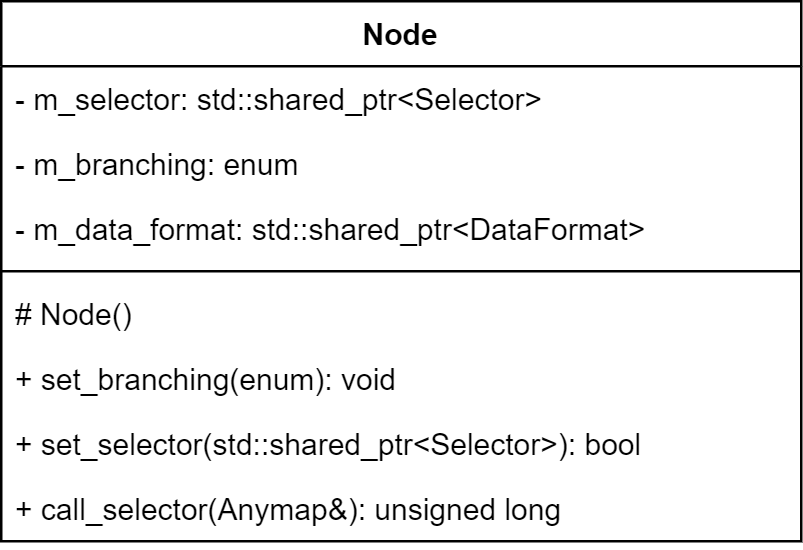
\includegraphics[width=\textwidth]{images/class.node.png}
		\caption{UML-диаграмма класса узла графа}
	\end{minipage}\hfill\begin{minipage}{0.49\textwidth}
		\centering
		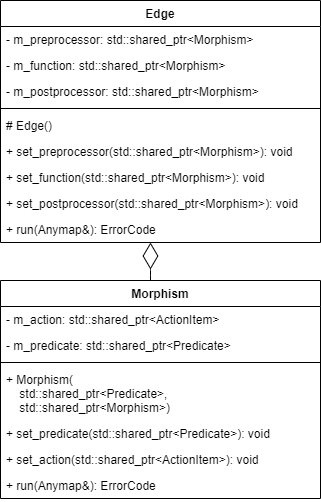
\includegraphics[scale=0.34]{images/class.edge.png}
		\caption{UML-диаграмма класса ребра графа}
	\end{minipage}\hfill
\end{figure}
\end{frame}
%%%%%%%%%%%%%%%%%%%%%%%%%%%%%%%%%%%%%%%%%%%%%%%
\subsection{Граф и обращение к его топологии}
%%%%%%%%%%%%%%%%%%%%%%%%%%%%%%%%%%%%%%%%%%%
\begin{frame}%[allowframebreaks=0.9,t]
	\begin{figure}
		\centering
		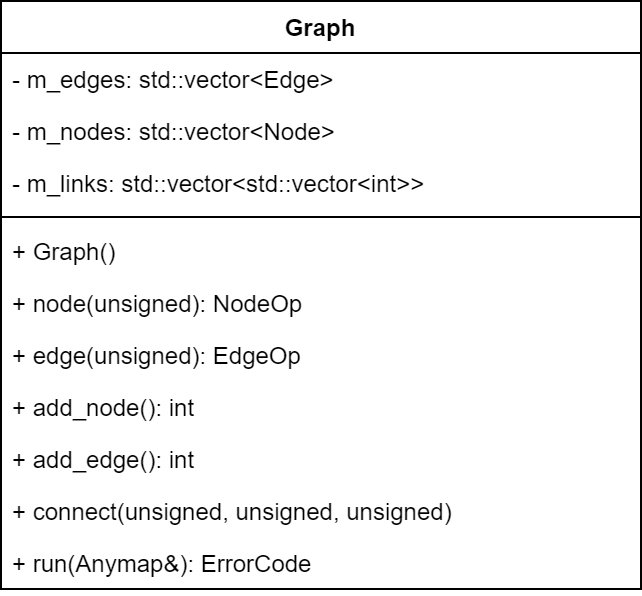
\includegraphics[scale=0.5]{images/class.graph.png}
		\caption{UML-диаграмма класса графа}
	\end{figure}
\end{frame}

\begin{frame}
	\begin{figure}
		\centering
		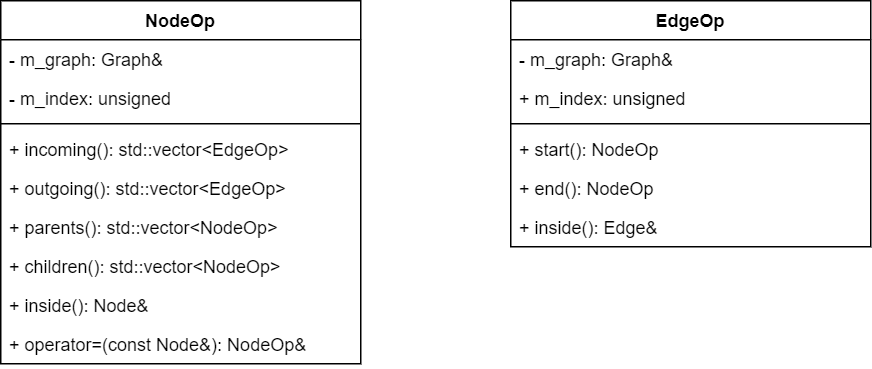
\includegraphics[width=\textwidth]{images/structure_additional.png}
		\caption{UML-диаграмма дополнительных структур данных}
	\end{figure}
\end{frame}
%%%%%%%%%%%%%%%%%%%%%%%%%%%%%%%%%%%%%%%%%%%%%%%
